\documentclass[]{article}
\usepackage{lmodern}
\usepackage{amssymb,amsmath}
\usepackage{ifxetex,ifluatex}
\usepackage{fixltx2e} % provides \textsubscript
\ifnum 0\ifxetex 1\fi\ifluatex 1\fi=0 % if pdftex
  \usepackage[T1]{fontenc}
  \usepackage[utf8]{inputenc}
\else % if luatex or xelatex
  \ifxetex
    \usepackage{mathspec}
  \else
    \usepackage{fontspec}
  \fi
  \defaultfontfeatures{Ligatures=TeX,Scale=MatchLowercase}
\fi
% use upquote if available, for straight quotes in verbatim environments
\IfFileExists{upquote.sty}{\usepackage{upquote}}{}
% use microtype if available
\IfFileExists{microtype.sty}{%
\usepackage{microtype}
\UseMicrotypeSet[protrusion]{basicmath} % disable protrusion for tt fonts
}{}
\usepackage[margin=1in]{geometry}
\usepackage{hyperref}
\hypersetup{unicode=true,
            pdftitle={Processing, cleaning and saving NZ GREEN Grid project 1 minute electricity power data},
            pdfauthor={Ben Anderson (b.anderson@soton.ac.uk, @dataknut)},
            pdfborder={0 0 0},
            breaklinks=true}
\urlstyle{same}  % don't use monospace font for urls
\usepackage{color}
\usepackage{fancyvrb}
\newcommand{\VerbBar}{|}
\newcommand{\VERB}{\Verb[commandchars=\\\{\}]}
\DefineVerbatimEnvironment{Highlighting}{Verbatim}{commandchars=\\\{\}}
% Add ',fontsize=\small' for more characters per line
\usepackage{framed}
\definecolor{shadecolor}{RGB}{248,248,248}
\newenvironment{Shaded}{\begin{snugshade}}{\end{snugshade}}
\newcommand{\KeywordTok}[1]{\textcolor[rgb]{0.13,0.29,0.53}{\textbf{#1}}}
\newcommand{\DataTypeTok}[1]{\textcolor[rgb]{0.13,0.29,0.53}{#1}}
\newcommand{\DecValTok}[1]{\textcolor[rgb]{0.00,0.00,0.81}{#1}}
\newcommand{\BaseNTok}[1]{\textcolor[rgb]{0.00,0.00,0.81}{#1}}
\newcommand{\FloatTok}[1]{\textcolor[rgb]{0.00,0.00,0.81}{#1}}
\newcommand{\ConstantTok}[1]{\textcolor[rgb]{0.00,0.00,0.00}{#1}}
\newcommand{\CharTok}[1]{\textcolor[rgb]{0.31,0.60,0.02}{#1}}
\newcommand{\SpecialCharTok}[1]{\textcolor[rgb]{0.00,0.00,0.00}{#1}}
\newcommand{\StringTok}[1]{\textcolor[rgb]{0.31,0.60,0.02}{#1}}
\newcommand{\VerbatimStringTok}[1]{\textcolor[rgb]{0.31,0.60,0.02}{#1}}
\newcommand{\SpecialStringTok}[1]{\textcolor[rgb]{0.31,0.60,0.02}{#1}}
\newcommand{\ImportTok}[1]{#1}
\newcommand{\CommentTok}[1]{\textcolor[rgb]{0.56,0.35,0.01}{\textit{#1}}}
\newcommand{\DocumentationTok}[1]{\textcolor[rgb]{0.56,0.35,0.01}{\textbf{\textit{#1}}}}
\newcommand{\AnnotationTok}[1]{\textcolor[rgb]{0.56,0.35,0.01}{\textbf{\textit{#1}}}}
\newcommand{\CommentVarTok}[1]{\textcolor[rgb]{0.56,0.35,0.01}{\textbf{\textit{#1}}}}
\newcommand{\OtherTok}[1]{\textcolor[rgb]{0.56,0.35,0.01}{#1}}
\newcommand{\FunctionTok}[1]{\textcolor[rgb]{0.00,0.00,0.00}{#1}}
\newcommand{\VariableTok}[1]{\textcolor[rgb]{0.00,0.00,0.00}{#1}}
\newcommand{\ControlFlowTok}[1]{\textcolor[rgb]{0.13,0.29,0.53}{\textbf{#1}}}
\newcommand{\OperatorTok}[1]{\textcolor[rgb]{0.81,0.36,0.00}{\textbf{#1}}}
\newcommand{\BuiltInTok}[1]{#1}
\newcommand{\ExtensionTok}[1]{#1}
\newcommand{\PreprocessorTok}[1]{\textcolor[rgb]{0.56,0.35,0.01}{\textit{#1}}}
\newcommand{\AttributeTok}[1]{\textcolor[rgb]{0.77,0.63,0.00}{#1}}
\newcommand{\RegionMarkerTok}[1]{#1}
\newcommand{\InformationTok}[1]{\textcolor[rgb]{0.56,0.35,0.01}{\textbf{\textit{#1}}}}
\newcommand{\WarningTok}[1]{\textcolor[rgb]{0.56,0.35,0.01}{\textbf{\textit{#1}}}}
\newcommand{\AlertTok}[1]{\textcolor[rgb]{0.94,0.16,0.16}{#1}}
\newcommand{\ErrorTok}[1]{\textcolor[rgb]{0.64,0.00,0.00}{\textbf{#1}}}
\newcommand{\NormalTok}[1]{#1}
\usepackage{longtable,booktabs}
\usepackage{graphicx,grffile}
\makeatletter
\def\maxwidth{\ifdim\Gin@nat@width>\linewidth\linewidth\else\Gin@nat@width\fi}
\def\maxheight{\ifdim\Gin@nat@height>\textheight\textheight\else\Gin@nat@height\fi}
\makeatother
% Scale images if necessary, so that they will not overflow the page
% margins by default, and it is still possible to overwrite the defaults
% using explicit options in \includegraphics[width, height, ...]{}
\setkeys{Gin}{width=\maxwidth,height=\maxheight,keepaspectratio}
\IfFileExists{parskip.sty}{%
\usepackage{parskip}
}{% else
\setlength{\parindent}{0pt}
\setlength{\parskip}{6pt plus 2pt minus 1pt}
}
\setlength{\emergencystretch}{3em}  % prevent overfull lines
\providecommand{\tightlist}{%
  \setlength{\itemsep}{0pt}\setlength{\parskip}{0pt}}
\setcounter{secnumdepth}{5}
% Redefines (sub)paragraphs to behave more like sections
\ifx\paragraph\undefined\else
\let\oldparagraph\paragraph
\renewcommand{\paragraph}[1]{\oldparagraph{#1}\mbox{}}
\fi
\ifx\subparagraph\undefined\else
\let\oldsubparagraph\subparagraph
\renewcommand{\subparagraph}[1]{\oldsubparagraph{#1}\mbox{}}
\fi

%%% Use protect on footnotes to avoid problems with footnotes in titles
\let\rmarkdownfootnote\footnote%
\def\footnote{\protect\rmarkdownfootnote}

%%% Change title format to be more compact
\usepackage{titling}

% Create subtitle command for use in maketitle
\newcommand{\subtitle}[1]{
  \posttitle{
    \begin{center}\large#1\end{center}
    }
}

\setlength{\droptitle}{-2em}
  \title{Processing, cleaning and saving NZ GREEN Grid project 1 minute
electricity power data}
  \pretitle{\vspace{\droptitle}\centering\huge}
  \posttitle{\par}
  \author{Ben Anderson
(\href{mailto:b.anderson@soton.ac.uk}{\nolinkurl{b.anderson@soton.ac.uk}},
\texttt{@dataknut})}
  \preauthor{\centering\large\emph}
  \postauthor{\par}
  \predate{\centering\large\emph}
  \postdate{\par}
  \date{Last run at: 2018-05-15 18:33:59}

\usepackage{booktabs}
\usepackage{longtable}
\usepackage{array}
\usepackage{multirow}
\usepackage[table]{xcolor}
\usepackage{wrapfig}
\usepackage{float}
\usepackage{colortbl}
\usepackage{pdflscape}
\usepackage{tabu}
\usepackage{threeparttable}
\usepackage{threeparttablex}
\usepackage[normalem]{ulem}
\usepackage{makecell}

\begin{document}
\maketitle

{
\setcounter{tocdepth}{2}
\tableofcontents
}
\newpage

\section{Status}\label{status}

\begin{verbatim}
## [1] "Test data run using data from ~/Data/NZGreenGrid/gridspy/1min_orig/"
\end{verbatim}

\section{Citation}\label{citation}

If you wish to use any of the material from this report please cite as:

\begin{itemize}
\tightlist
\item
  Anderson, B. (2018) Processing, cleaning and saving NZ GREEN Grid
  project 1 minute electricity power data, University of Otago: Dunedin,
  NZ.
\end{itemize}

\newpage

\section{Introduction}\label{introduction}

Report circulation:

\begin{itemize}
\tightlist
\item
  Restricted to:
  \href{https://www.otago.ac.nz/centre-sustainability/research/energy/otago050285.html}{NZ
  GREEN Grid} project partners and contractors.
\end{itemize}

\subsection{Purpose}\label{purpose}

This report is intended to:

\begin{itemize}
\tightlist
\item
  load and clean the project electricity power data (Grid Spy)
\item
  save the cleaned data out as a single file per household
\item
  produce summary data quality statistics
\end{itemize}

The resulting cleaned data has \emph{no} identifying information such as
names, addresses, email addresses, telephone numbers and is therefore
safe to share across all partners.

The data contains a unique household id which can be used to link it to
the NZ GREEN Grid time use diaries and dwelling/appliance surveys. With
some additional non-disclosure checks it should also be safe to archive
all of these linkable datasets for re-use via the UK
\href{http://reshare.ukdataservice.ac.uk/}{reshare} service.

\subsection{Requirements:}\label{requirements}

\begin{itemize}
\tightlist
\item
  grid spy 1 minute data downloads
\end{itemize}

\subsection{History}\label{history}

Generally tracked via our git.soton
\href{https://git.soton.ac.uk/ba1e12/nzGREENGrid}{repo}:

\begin{itemize}
\tightlist
\item
  \href{https://git.soton.ac.uk/ba1e12/nzGREENGrid/commits/master}{history}
\item
  \href{https://git.soton.ac.uk/ba1e12/nzGREENGrid/issues}{issues}
\end{itemize}

\subsection{Support}\label{support}

This work was supported by:

\begin{itemize}
\tightlist
\item
  The \href{https://www.otago.ac.nz/}{University of Otago}
\item
  The New Zealand \href{http://www.mbie.govt.nz/}{Ministry of Business,
  Innovation and Employment (MBIE)}
\item
  \href{http://www.energy.soton.ac.uk/tag/spatialec/}{SPATIALEC} - a
  \href{http://ec.europa.eu/research/mariecurieactions/about-msca/actions/if/index_en.htm}{Marie
  Skłodowska-Curie Global Fellowship} based at the University of Otago's
  \href{http://www.otago.ac.nz/centre-sustainability/staff/otago673896.html}{Centre
  for Sustainability} (2017-2019) \& the University of Southampton's
  Sustainable Energy Research Group (2019-202).
\end{itemize}

This work is (c) 2018 the University of Southampton.

We do not `support' the code but if you have a problem check the
\href{https://git.soton.ac.uk/ba1e12/nzGREENGrid/issues}{issues} on our
\href{https://git.soton.ac.uk/ba1e12/nzGREENGrid}{repo} and if it
doesn't already exist, open one. We might be able to fix it :-)

\section{Obtain listing of files}\label{obtain-listing-of-files}

In this section we generate a listing of all 1 minute data files that we
have received. If we are running over the complete dataset then we will
be using data from:

\begin{itemize}
\tightlist
\item
  /hum-csafe/Research Projects/GREEN Grid/\_RAW DATA/GridSpyData/
\end{itemize}

In this run we are using data from:

\begin{itemize}
\tightlist
\item
  \textasciitilde{}/Data/NZGreenGrid/gridspy/1min\_orig/
\end{itemize}

If these do not match then this may be a test run.

\begin{Shaded}
\begin{Highlighting}[]
\KeywordTok{source}\NormalTok{(}\StringTok{"../scripts/process1minGridSpyFiles.R"}\NormalTok{)}
\end{Highlighting}
\end{Shaded}

\begin{verbatim}
## Loading required package: data.table
\end{verbatim}

\begin{verbatim}
## Loading required package: lubridate
\end{verbatim}

\begin{verbatim}
## 
## Attaching package: 'lubridate'
\end{verbatim}

\begin{verbatim}
## The following objects are masked from 'package:data.table':
## 
##     hour, isoweek, mday, minute, month, quarter, second, wday,
##     week, yday, year
\end{verbatim}

\begin{verbatim}
## The following object is masked from 'package:base':
## 
##     date
\end{verbatim}

\begin{verbatim}
## Loading required package: readr
\end{verbatim}

\begin{verbatim}
## Loading required package: dplyr
\end{verbatim}

\begin{verbatim}
## 
## Attaching package: 'dplyr'
\end{verbatim}

\begin{verbatim}
## The following objects are masked from 'package:lubridate':
## 
##     intersect, setdiff, union
\end{verbatim}

\begin{verbatim}
## The following objects are masked from 'package:data.table':
## 
##     between, first, last
\end{verbatim}

\begin{verbatim}
## The following object is masked from 'package:ggplot2':
## 
##     vars
\end{verbatim}

\begin{verbatim}
## The following objects are masked from 'package:stats':
## 
##     filter, lag
\end{verbatim}

\begin{verbatim}
## The following objects are masked from 'package:base':
## 
##     intersect, setdiff, setequal, union
\end{verbatim}

\begin{verbatim}
## Loading required package: progress
\end{verbatim}

\begin{verbatim}
## [1] "Looking for 1 minute data using pattern = *at1.csv$ in ~/Data/NZGreenGrid/gridspy/1min_orig/ - could take a while..."
## [1] "Looking for data using pattern = *at1.csv$ in ~/Data/NZGreenGrid/gridspy/1min_orig/ - could take a while..."
## [1] "Found 958 files"
## [1] "Processing file list and getting file meta-data (please be patient)"
## [1] "All files checked"
## [1] "Checking ambiguous date formats in ~/Data/NZGreenGrid/gridspy/1min_orig/rf_46/12Oct2016-20Nov2017at1.csv"
## [1] "Saving 1 minute data files interim metadata to ~/Data/NZGreenGrid/gridspy/consolidated/1min/fListCompleteDT_interim.csv"
## [1] "Done"
\end{verbatim}

\begin{Shaded}
\begin{Highlighting}[]
\KeywordTok{print}\NormalTok{(}\KeywordTok{paste0}\NormalTok{(}\StringTok{"Overall we have "}\NormalTok{, }\KeywordTok{nrow}\NormalTok{(fListCompleteDT), }\StringTok{" files from "}\NormalTok{, }\KeywordTok{uniqueN}\NormalTok{(fListCompleteDT}\OperatorTok{$}\NormalTok{hhID), }\StringTok{" households."}\NormalTok{))}
\end{Highlighting}
\end{Shaded}

\begin{verbatim}
## [1] "Overall we have 958 files from 2 households."
\end{verbatim}

\begin{Shaded}
\begin{Highlighting}[]
\CommentTok{# for use below}
\NormalTok{nFiles <-}\StringTok{ }\KeywordTok{nrow}\NormalTok{(fListCompleteDT)}
\NormalTok{nFilesNotLoaded <-}\StringTok{ }\KeywordTok{nrow}\NormalTok{(fListCompleteDT[dateColName }\OperatorTok\StringTok{ "unknown"}\NormalTok{])}
\end{Highlighting}
\end{Shaded}

Overall we have 958 files from 2 households. Of the 958, 544 (56.78\%)
were \emph{not} loaded/checked as their file sizes indicated that they
contained no data.

\subsection{Date format checks}\label{date-format-checks}

We now need to check how many of the loaded files have an ambiguous or
default date - these could introduce errors.

\begin{Shaded}
\begin{Highlighting}[]
\CommentTok{# short cut if interim file list already saved ----}
\CommentTok{#ifile <- paste0(outPath, fListInterim)}
\CommentTok{#print(paste0("Loading 1 minute data files interim metadata to ", ifile))}
\CommentTok{#fListCompleteDT <- fread(ifile)}
  
  
\NormalTok{t <-}\StringTok{ }\NormalTok{fListCompleteDT[, .(}\DataTypeTok{nFiles =}\NormalTok{ .N, }
                         \DataTypeTok{minDate =} \KeywordTok{min}\NormalTok{(dateExample), }\CommentTok{# may not make much sense}
                         \DataTypeTok{maxDate =} \KeywordTok{max}\NormalTok{(dateExample)), keyby =}\StringTok{ }\NormalTok{.(dateColName, dateFormat)]}

\NormalTok{knitr}\OperatorTok{::}\KeywordTok{kable}\NormalTok{(t, }
             \DataTypeTok{caption =} \StringTok{"Number of files and min/max date (as char) with given date column names by inferred date format"}\NormalTok{, }
             \DataTypeTok{format =} \StringTok{"latex"}\NormalTok{, }
             \DataTypeTok{booktabs =}\NormalTok{ T) }\OperatorTok
\StringTok{  }\KeywordTok{kable_styling}\NormalTok{(}\DataTypeTok{font_size =} \DecValTok{8}\NormalTok{)}
\end{Highlighting}
\end{Shaded}

\begin{table}

\caption{\label{tab:initialDateFormatTable}Number of files and min/max date (as char) with given date column names by inferred date format}
\centering
\fontsize{8}{10}\selectfont
\begin{tabular}[t]{llrll}
\toprule
dateColName & dateFormat & nFiles & minDate & maxDate\\
\midrule
date NZ & dmy - definite & 1 & 27/03/2015 & 27/03/2015\\
date NZ & mdy - definite & 1 & 5/26/2016 & 5/26/2016\\
date NZ & ymd - default (but day/month value <= 12) & 1 & 2014-01-06 & 2014-01-06\\
date NZ & ymd - definite & 2 & 2014-05-24 & 2015-05-25\\
date UTC & ambiguous & 1 & 11-10-16 & 11-10-16\\
\addlinespace
date UTC & ymd - default (but day/month value <= 12) & 161 & 2017-01-08 & 2018-02-12\\
date UTC & ymd - definite & 247 & 2015-05-24 & 2018-02-19\\
unknown - do not load (fsize = 2751) & NA & 302 & NA & NA\\
unknown - do not load (fsize = 43) & NA & 242 & NA & NA\\
\bottomrule
\end{tabular}
\end{table}

Results to note:

\begin{itemize}
\tightlist
\item
  There are 1 ambiguous files
\item
  The non-loaded files only have 2 distinct file sizes, confirming that
  they are unlikely to contain useful data.
\end{itemize}

We now inspect the ambiguous and (some of) the default files.

To help with data cleaning the following table lists files that have
ambiguous dates.

\begin{Shaded}
\begin{Highlighting}[]
\CommentTok{# list ambigious files}
\NormalTok{aList <-}\StringTok{ }\NormalTok{fListCompleteDT[dateFormat }\OperatorTok{==}\StringTok{ "ambiguous"}\NormalTok{, .(file, dateColName, dateExample, dateFormat)]}

\NormalTok{cap <-}\StringTok{ }\KeywordTok{paste0}\NormalTok{(}\StringTok{"All "}\NormalTok{, }\KeywordTok{nrow}\NormalTok{(aList), }\StringTok{" files with an ambiguous dateFormat"}\NormalTok{)}

\NormalTok{knitr}\OperatorTok{::}\KeywordTok{kable}\NormalTok{(}\DataTypeTok{caption =}\NormalTok{ cap, aList)}
\end{Highlighting}
\end{Shaded}

\begin{longtable}[]{@{}llll@{}}
\caption{All 1 files with an ambiguous dateFormat}\tabularnewline
\toprule
file & dateColName & dateExample & dateFormat\tabularnewline
\midrule
\endfirsthead
\toprule
file & dateColName & dateExample & dateFormat\tabularnewline
\midrule
\endhead
rf\_46/12Oct2016-20Nov2017at1.csv & date UTC & 11-10-16 &
ambiguous\tabularnewline
\bottomrule
\end{longtable}

Check against file names to see what is reasonable and then fix them.

\begin{Shaded}
\begin{Highlighting}[]
\CommentTok{# Setting to dmy seems OK}
\NormalTok{fListCompleteDT <-}\StringTok{ }\NormalTok{fListCompleteDT[dateFormat }\OperatorTok{==}\StringTok{ "ambiguous"}\NormalTok{, dateFormat }\OperatorTok{:}\ErrorTok{=}\StringTok{ "dmy - inferred"}\NormalTok{]}

\KeywordTok{paste0}\NormalTok{(}\StringTok{"Fixed "}\NormalTok{, }\KeywordTok{nrow}\NormalTok{(aList), }\StringTok{" files with an ambiguous dateFormat"}\NormalTok{)}
\end{Highlighting}
\end{Shaded}

\begin{verbatim}
## [1] "Fixed 1 files with an ambiguous dateFormat"
\end{verbatim}

The following table lists up to 10 of the `date NZ' files which are set
by default - do they look OK to assume the default dateFormat? Compare
the file names with the dateExample\ldots{}

\begin{Shaded}
\begin{Highlighting}[]
\CommentTok{# list default files}
\NormalTok{aList <-}\StringTok{ }\NormalTok{fListCompleteDT[dateColName }\OperatorTok{==}\StringTok{ "date NZ"} \OperatorTok{&}\StringTok{ }\NormalTok{dateFormat }\OperatorTok\StringTok{ "default"}\NormalTok{, .(file, fSize, dateColName, dateExample, dateFormat)]}

\NormalTok{cap <-}\StringTok{ }\KeywordTok{paste0}\NormalTok{(}\StringTok{"First 10 (max) of "}\NormalTok{, }\KeywordTok{nrow}\NormalTok{(aList), }\StringTok{" files with dateColName = 'date NZ' and default dateFormat"}\NormalTok{)}

\NormalTok{knitr}\OperatorTok{::}\KeywordTok{kable}\NormalTok{(}\DataTypeTok{caption =}\NormalTok{ cap, }\KeywordTok{head}\NormalTok{(aList))}
\end{Highlighting}
\end{Shaded}

\begin{longtable}[]{@{}lrlll@{}}
\caption{First 10 (max) of 1 files with dateColName = `date NZ' and
default dateFormat}\tabularnewline
\toprule
file & fSize & dateColName & dateExample & dateFormat\tabularnewline
\midrule
\endfirsthead
\toprule
file & fSize & dateColName & dateExample & dateFormat\tabularnewline
\midrule
\endhead
rf\_01/1Jan2014-24May2014at1.csv & 6255737 & date NZ & 2014-01-06 & ymd
- default (but day/month value \textless{}= 12)\tabularnewline
\bottomrule
\end{longtable}

The following table lists up to 10 of the `date UTC' files which are set
by default - do they look OK to assume the default dateFormat? Compare
the file names with the dateExample\ldots{}

\begin{Shaded}
\begin{Highlighting}[]
\CommentTok{# list default files}
\NormalTok{aList <-}\StringTok{ }\NormalTok{fListCompleteDT[dateColName }\OperatorTok{==}\StringTok{ "date UTC"} \OperatorTok{&}\StringTok{ }\NormalTok{dateFormat }\OperatorTok\StringTok{ "default"}\NormalTok{, .(file, fSize, dateColName, dateExample, dateFormat)]}

\NormalTok{cap <-}\StringTok{ }\KeywordTok{paste0}\NormalTok{(}\StringTok{"First 10 (max) of "}\NormalTok{, }\KeywordTok{nrow}\NormalTok{(aList), }\StringTok{" files with dateColName = 'date UTC' and default dateFormat"}\NormalTok{)}

\NormalTok{knitr}\OperatorTok{::}\KeywordTok{kable}\NormalTok{(}\DataTypeTok{caption =}\NormalTok{ cap, }\KeywordTok{head}\NormalTok{(aList, }\DecValTok{10}\NormalTok{))}
\end{Highlighting}
\end{Shaded}

\begin{longtable}[]{@{}lrlll@{}}
\caption{First 10 (max) of 161 files with dateColName = `date UTC' and
default dateFormat}\tabularnewline
\toprule
file & fSize & dateColName & dateExample & dateFormat\tabularnewline
\midrule
\endfirsthead
\toprule
file & fSize & dateColName & dateExample & dateFormat\tabularnewline
\midrule
\endhead
rf\_46/10Apr2017-11Apr2017at1.csv & 292721 & date UTC & 2017-04-09 & ymd
- default (but day/month value \textless{}= 12)\tabularnewline
rf\_46/10Aug2017-11Aug2017at1.csv & 292888 & date UTC & 2017-08-09 & ymd
- default (but day/month value \textless{}= 12)\tabularnewline
rf\_46/10Dec2017-11Dec2017at1.csv & 292823 & date UTC & 2017-12-09 & ymd
- default (but day/month value \textless{}= 12)\tabularnewline
rf\_46/10Feb2017-11Feb2017at1.csv & 286736 & date UTC & 2017-02-09 & ymd
- default (but day/month value \textless{}= 12)\tabularnewline
rf\_46/10Feb2018-11Feb2018at1.csv & 299084 & date UTC & 2018-02-09 & ymd
- default (but day/month value \textless{}= 12)\tabularnewline
rf\_46/10Jan2017-11Jan2017at1.csv & 297659 & date UTC & 2017-01-09 & ymd
- default (but day/month value \textless{}= 12)\tabularnewline
rf\_46/10Jan2018-11Jan2018at1.csv & 294418 & date UTC & 2018-01-09 & ymd
- default (but day/month value \textless{}= 12)\tabularnewline
rf\_46/10Jul2017-11Jul2017at1.csv & 291082 & date UTC & 2017-07-09 & ymd
- default (but day/month value \textless{}= 12)\tabularnewline
rf\_46/10Jun2017-11Jun2017at1.csv & 295979 & date UTC & 2017-06-09 & ymd
- default (but day/month value \textless{}= 12)\tabularnewline
rf\_46/10Mar2017-11Mar2017at1.csv & 290244 & date UTC & 2017-03-09 & ymd
- default (but day/month value \textless{}= 12)\tabularnewline
\bottomrule
\end{longtable}

Check final date formats:

\begin{Shaded}
\begin{Highlighting}[]
\NormalTok{t <-}\StringTok{ }\NormalTok{fListCompleteDT[, .(}\DataTypeTok{nFiles =}\NormalTok{ .N, }
                         \DataTypeTok{minDate =} \KeywordTok{min}\NormalTok{(dateExample), }\CommentTok{# may not make much sense}
                         \DataTypeTok{maxDate =} \KeywordTok{max}\NormalTok{(dateExample)), keyby =}\StringTok{ }\NormalTok{.(dateColName, dateFormat)]}

\NormalTok{knitr}\OperatorTok{::}\KeywordTok{kable}\NormalTok{(}\DataTypeTok{caption =} \StringTok{"Number of files & min/max dates (as char) with given date column names by final imputed date format"}\NormalTok{, t)}
\end{Highlighting}
\end{Shaded}

\begin{longtable}[]{@{}llrll@{}}
\caption{Number of files \& min/max dates (as char) with given date
column names by final imputed date format}\tabularnewline
\toprule
dateColName & dateFormat & nFiles & minDate & maxDate\tabularnewline
\midrule
\endfirsthead
\toprule
dateColName & dateFormat & nFiles & minDate & maxDate\tabularnewline
\midrule
\endhead
date NZ & dmy - definite & 1 & 27/03/2015 & 27/03/2015\tabularnewline
date NZ & mdy - definite & 1 & 5/26/2016 & 5/26/2016\tabularnewline
date NZ & ymd - default (but day/month value \textless{}= 12) & 1 &
2014-01-06 & 2014-01-06\tabularnewline
date NZ & ymd - definite & 2 & 2014-05-24 & 2015-05-25\tabularnewline
date UTC & dmy - inferred & 1 & 11-10-16 & 11-10-16\tabularnewline
date UTC & ymd - default (but day/month value \textless{}= 12) & 161 &
2017-01-08 & 2018-02-12\tabularnewline
date UTC & ymd - definite & 247 & 2015-05-24 & 2018-02-19\tabularnewline
unknown - do not load (fsize = 2751) & NA & 302 & NA & NA\tabularnewline
unknown - do not load (fsize = 43) & NA & 242 & NA & NA\tabularnewline
\bottomrule
\end{longtable}

\subsection{Data file quality checks}\label{data-file-quality-checks}

The following chart shows the distribution of these files over time
using their sizes. Note that white indicates the presence of small files
which may not contain observations.

\begin{Shaded}
\begin{Highlighting}[]
\NormalTok{myCaption <-}\StringTok{ }\KeywordTok{paste0}\NormalTok{(}\StringTok{"Data source: "}\NormalTok{, fpath,}
                    \StringTok{"}\CharTok{\textbackslash{}n}\StringTok{Using data received up to "}\NormalTok{, }\KeywordTok{Sys.Date}\NormalTok{())}

\NormalTok{plotDT <-}\StringTok{ }\NormalTok{fListCompleteDT[, .(}\DataTypeTok{nFiles =}\NormalTok{ .N,}
                              \DataTypeTok{meanfSize =} \KeywordTok{mean}\NormalTok{(fSize)), }
\NormalTok{                          keyby =}\StringTok{ }\NormalTok{.(hhID, }\DataTypeTok{date =} \KeywordTok{as.Date}\NormalTok{(fMDate))]}

\NormalTok{ggplot2}\OperatorTok{::}\KeywordTok{ggplot}\NormalTok{(plotDT, }\KeywordTok{aes}\NormalTok{( }\DataTypeTok{x =}\NormalTok{ date, }\DataTypeTok{y =}\NormalTok{ hhID, }\DataTypeTok{fill =} \KeywordTok{log}\NormalTok{(meanfSize))) }\OperatorTok{+}
\StringTok{  }\KeywordTok{geom_tile}\NormalTok{() }\OperatorTok{+}
\StringTok{  }\KeywordTok{scale_fill_gradient}\NormalTok{(}\DataTypeTok{low =} \StringTok{"white"}\NormalTok{, }\DataTypeTok{high =} \StringTok{"black"}\NormalTok{) }\OperatorTok{+}\StringTok{ }
\StringTok{  }\KeywordTok{scale_x_date}\NormalTok{(}\DataTypeTok{date_labels =} \StringTok{"%Y %b"}\NormalTok{, }\DataTypeTok{date_breaks =} \StringTok{"1 month"}\NormalTok{) }\OperatorTok{+}
\StringTok{  }\KeywordTok{theme}\NormalTok{(}\DataTypeTok{axis.text.x =} \KeywordTok{element_text}\NormalTok{(}\DataTypeTok{angle =} \DecValTok{90}\NormalTok{, }\DataTypeTok{vjust =} \FloatTok{0.5}\NormalTok{, }\DataTypeTok{hjust =} \FloatTok{0.5}\NormalTok{)) }\OperatorTok{+}\StringTok{ }
\StringTok{  }\KeywordTok{labs}\NormalTok{(}\DataTypeTok{title =} \StringTok{"Mean file size of all grid spy data files received per day"}\NormalTok{,}
       \DataTypeTok{caption =} \KeywordTok{paste0}\NormalTok{(myCaption, }
                        \StringTok{"}\CharTok{\textbackslash{}n}\StringTok{Log file size used as some files are full year data"}\NormalTok{)}
    
\NormalTok{  )}
\end{Highlighting}
\end{Shaded}

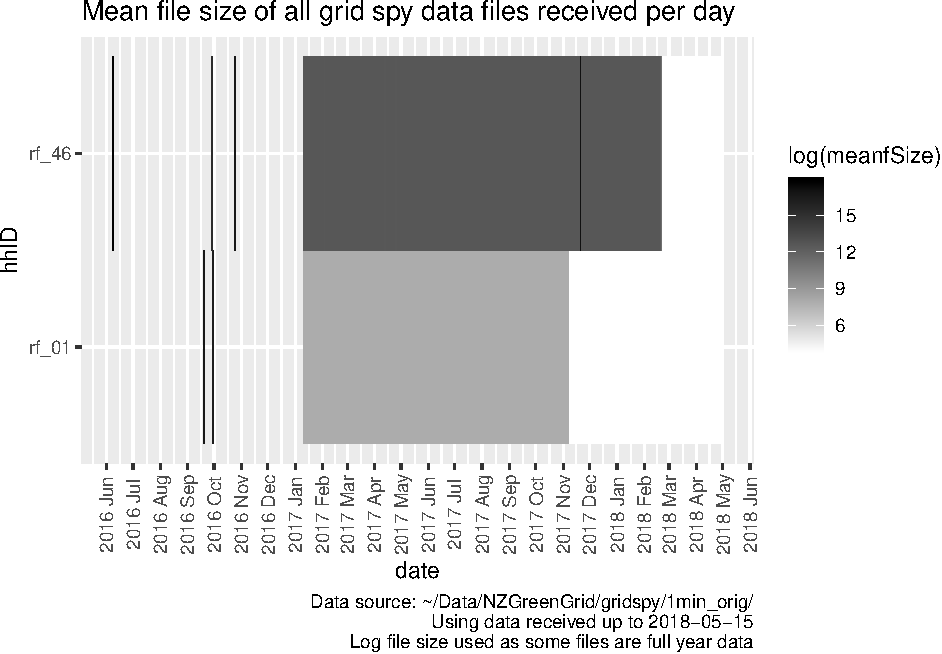
\includegraphics{processNZGGElecCons1minData_v2_files/figure-latex/allFileSizesPlot-1.pdf}

\begin{Shaded}
\begin{Highlighting}[]
\NormalTok{ggplot2}\OperatorTok{::}\KeywordTok{ggsave}\NormalTok{(}\KeywordTok{paste0}\NormalTok{(outPath, }\StringTok{"gridSpyAllFileListSizeTilePlot.png"}\NormalTok{))}
\end{Highlighting}
\end{Shaded}

\begin{verbatim}
## Saving 6.5 x 4.5 in image
\end{verbatim}

The following chart shows the same chart but only for files which we
think contain data.

\begin{Shaded}
\begin{Highlighting}[]
\NormalTok{myCaption <-}\StringTok{ }\KeywordTok{paste0}\NormalTok{(}\StringTok{"Data source: "}\NormalTok{, fpath,}
                    \StringTok{"}\CharTok{\textbackslash{}n}\StringTok{Using data received up to "}\NormalTok{, }\KeywordTok{Sys.Date}\NormalTok{())}

\NormalTok{plotDT <-}\StringTok{ }\NormalTok{fListCompleteDT[}\OperatorTok{!}\KeywordTok{is.na}\NormalTok{(dateFormat), .(}\DataTypeTok{nFiles =}\NormalTok{ .N,}
                              \DataTypeTok{meanfSize =} \KeywordTok{mean}\NormalTok{(fSize)), }
\NormalTok{                          keyby =}\StringTok{ }\NormalTok{.(hhID, }\DataTypeTok{date =} \KeywordTok{as.Date}\NormalTok{(fMDate))]}

\NormalTok{ggplot2}\OperatorTok{::}\KeywordTok{ggplot}\NormalTok{(plotDT, }\KeywordTok{aes}\NormalTok{( }\DataTypeTok{x =}\NormalTok{ date, }\DataTypeTok{y =}\NormalTok{ hhID, }\DataTypeTok{fill =} \KeywordTok{log}\NormalTok{(meanfSize))) }\OperatorTok{+}
\StringTok{  }\KeywordTok{geom_tile}\NormalTok{() }\OperatorTok{+}
\StringTok{  }\KeywordTok{scale_fill_gradient}\NormalTok{(}\DataTypeTok{low =} \StringTok{"white"}\NormalTok{, }\DataTypeTok{high =} \StringTok{"black"}\NormalTok{) }\OperatorTok{+}\StringTok{ }
\StringTok{  }\KeywordTok{scale_x_date}\NormalTok{(}\DataTypeTok{date_labels =} \StringTok{"%Y %b"}\NormalTok{, }\DataTypeTok{date_breaks =} \StringTok{"1 month"}\NormalTok{) }\OperatorTok{+}
\StringTok{  }\KeywordTok{theme}\NormalTok{(}\DataTypeTok{axis.text.x =} \KeywordTok{element_text}\NormalTok{(}\DataTypeTok{angle =} \DecValTok{90}\NormalTok{, }\DataTypeTok{vjust =} \FloatTok{0.5}\NormalTok{, }\DataTypeTok{hjust =} \FloatTok{0.5}\NormalTok{)) }\OperatorTok{+}\StringTok{ }
\StringTok{  }\KeywordTok{labs}\NormalTok{(}\DataTypeTok{title =} \StringTok{"Mean file size of loaded grid spy data files received per day"}\NormalTok{,}
       \DataTypeTok{caption =} \KeywordTok{paste0}\NormalTok{(myCaption, }
                        \StringTok{"}\CharTok{\textbackslash{}n}\StringTok{Log file size used as some files are full year data"}\NormalTok{,}
                        \StringTok{"}\CharTok{\textbackslash{}n}\StringTok{Files loaded if fsize > "}\NormalTok{, dataThreshold, }\StringTok{" bytes"}\NormalTok{)}
    
\NormalTok{  )}
\end{Highlighting}
\end{Shaded}

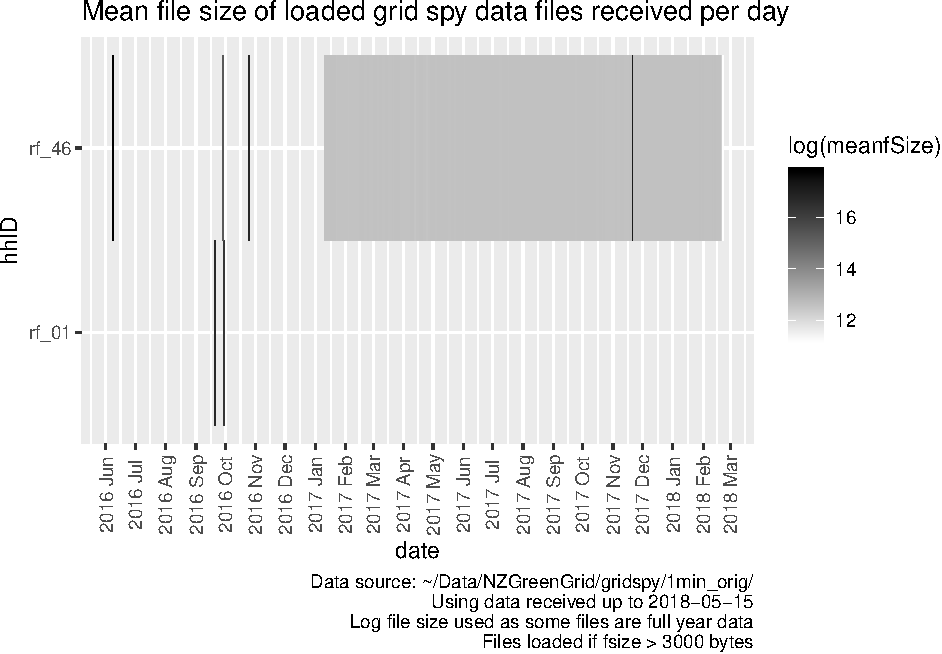
\includegraphics{processNZGGElecCons1minData_v2_files/figure-latex/loadedFileSizesPlot-1.pdf}

\begin{Shaded}
\begin{Highlighting}[]
\NormalTok{ggplot2}\OperatorTok{::}\KeywordTok{ggsave}\NormalTok{(}\KeywordTok{paste0}\NormalTok{(outPath, }\StringTok{"gridSpyLoadedFileListSizeTilePlot.png"}\NormalTok{))}
\end{Highlighting}
\end{Shaded}

\begin{verbatim}
## Saving 6.5 x 4.5 in image
\end{verbatim}

\section{Load data files}\label{load-data-files}

In this section we load the data files that have a file size
\textgreater{} 3000 bytes. Things to note:

\begin{itemize}
\tightlist
\item
  We assume that any files smaller than this value have no observations.
  This is based on:

  \begin{itemize}
  \tightlist
  \item
    Manual inspection of several small files
  \item
    The identical (small) file sizes involved
  \item
    \emph{But} we should probably test the first few lines to double
    check\ldots{}
  \end{itemize}
\item
  We have to deal with quite a lot of duplication some of which has
  caused the different date formats. See our
  \href{https://git.soton.ac.uk/ba1e12/nzGREENGrid/issues?scope=all\&utf8=\%E2\%9C\%93\&state=all}{repo
  issues list}.
\end{itemize}

The following table shows the number of files per household that we
willl load.

\begin{Shaded}
\begin{Highlighting}[]
\NormalTok{t <-}\StringTok{ }\NormalTok{fListCompleteDT[dateColName }\OperatorTok\StringTok{ "do not load"}\NormalTok{, .(}\DataTypeTok{nFiles =}\NormalTok{ .N,}
                       \DataTypeTok{meanSize =} \KeywordTok{mean}\NormalTok{(fSize),}
                       \DataTypeTok{minFileDate =} \KeywordTok{min}\NormalTok{(fMDate),}
                       \DataTypeTok{maxFileDate =} \KeywordTok{max}\NormalTok{(fMDate)), keyby =}\StringTok{ }\NormalTok{.(hhID)]}

\NormalTok{knitr}\OperatorTok{::}\KeywordTok{kable}\NormalTok{(}\DataTypeTok{caption =} \StringTok{"Summary of household files to load"}\NormalTok{, t)}
\end{Highlighting}
\end{Shaded}

\begin{longtable}[]{@{}lrrll@{}}
\caption{Summary of household files to load}\tabularnewline
\toprule
hhID & nFiles & meanSize & minFileDate & maxFileDate\tabularnewline
\midrule
\endfirsthead
\toprule
hhID & nFiles & meanSize & minFileDate & maxFileDate\tabularnewline
\midrule
\endhead
rf\_01 & 475 & 1764.718 & 2017-01-11 & 2018-04-29\tabularnewline
rf\_46 & 69 & 43.000 & 2018-02-22 & 2018-05-01\tabularnewline
\bottomrule
\end{longtable}

\begin{Shaded}
\begin{Highlighting}[]
\CommentTok{#load data here}
\KeywordTok{source}\NormalTok{(}\StringTok{"../scripts/process1minGridSpyData.R"}\NormalTok{)}
\end{Highlighting}
\end{Shaded}

\begin{verbatim}
## [1] "Loading: rf_01"
## [1] "Saving ~/Data/NZGreenGrid/gridspy/consolidated/1min/data/rf_01_all_1min_data.csv..."
## [1] "Saved ~/Data/NZGreenGrid/gridspy/consolidated/1min/data/rf_01_all_1min_data.csv, gzipping..."
## [1] "Gzipped ~/Data/NZGreenGrid/gridspy/consolidated/1min/data/rf_01_all_1min_data.csv"
## [1] "Loading: rf_46"
## [1] "Saving ~/Data/NZGreenGrid/gridspy/consolidated/1min/data/rf_46_all_1min_data.csv..."
## [1] "Saved ~/Data/NZGreenGrid/gridspy/consolidated/1min/data/rf_46_all_1min_data.csv, gzipping..."
## [1] "Gzipped ~/Data/NZGreenGrid/gridspy/consolidated/1min/data/rf_46_all_1min_data.csv"
## [1] "Saving daily observations stats by hhid to ~/Data/NZGreenGrid/gridspy/consolidated/1min/hhDailyObservationsStats.csv"
## [1] "Done"
## [1] "Saving 1 minute data files final metadata to ~/Data/NZGreenGrid/gridspy/consolidated/1min/fListCompleteDT_final.csv"
## [1] "Done"
\end{verbatim}

\section{Data quality analysis}\label{data-quality-analysis}

Now produce some data quality plots \& tables.

\subsection{Circuit label checks}\label{circuit-label-checks}

The following table shows the number of data files with different
circuit labels by household. In theory there should only be one unique
list per household and it should be present in every data file.

\begin{Shaded}
\begin{Highlighting}[]
\CommentTok{# short cut if exists already}
\CommentTok{#ifile <- paste0(outPath, fListFinal)}
\CommentTok{#fListCompleteDT <- fread(ifile)}
\NormalTok{t <-}\StringTok{ }\KeywordTok{table}\NormalTok{(fListCompleteDT}\OperatorTok{$}\NormalTok{hhID,fListCompleteDT}\OperatorTok{$}\NormalTok{circuitLabels)}
\NormalTok{knitr}\OperatorTok{::}\KeywordTok{kable}\NormalTok{(}\DataTypeTok{caption =} \StringTok{"Circuit labels list by household"}\NormalTok{, t)}
\end{Highlighting}
\end{Shaded}

\begin{longtable}[]{@{}lrr@{}}
\caption{Circuit labels list by household}\tabularnewline
\toprule
& Heat Pumps (2x) \& Power\$4232, Heat Pumps (2x) \& Power\$4399, Hot
Water - Controlled\$4231, Hot Water - Controlled\$4400, Incomer -
Uncontrolled\$4230, Incomer - Uncontrolled\$4401, Incomer Voltage\$4405,
Kitchen \& Bedrooms\$4229, Kitchen \& Bedrooms\$4402, Laundry \&
Bedrooms\$4228, Laundry \& Bedrooms\$4403, Lighting\$4233,
Lighting\$4404 & Heating\$1633, Hot water\$1636, Kitchen power\$1632,
Lights\$1635, Mains\$1634, Range\$1637\tabularnewline
\midrule
\endfirsthead
\toprule
& Heat Pumps (2x) \& Power\$4232, Heat Pumps (2x) \& Power\$4399, Hot
Water - Controlled\$4231, Hot Water - Controlled\$4400, Incomer -
Uncontrolled\$4230, Incomer - Uncontrolled\$4401, Incomer Voltage\$4405,
Kitchen \& Bedrooms\$4229, Kitchen \& Bedrooms\$4402, Laundry \&
Bedrooms\$4228, Laundry \& Bedrooms\$4403, Lighting\$4233,
Lighting\$4404 & Heating\$1633, Hot water\$1636, Kitchen power\$1632,
Lights\$1635, Mains\$1634, Range\$1637\tabularnewline
\midrule
\endhead
rf\_01 & 0 & 3\tabularnewline
rf\_46 & 411 & 0\tabularnewline
\bottomrule
\end{longtable}

If this is not the case then this implies that:

\begin{itemize}
\tightlist
\item
  some of the circuit labels for these households may have been changed
  during the data collection process;
\item
  some of the circuit labels may have character conversion errors which
  have changed the labels during the data collection process;
\item
  at least one file from one household has been saved to a folder
  containing data from a different household (unfortunately the raw data
  files do \emph{not} contain household IDs in the data or the file
  names which would enable checking/preventative filtering). This will
  be visible in the table if two households appear to share
  \emph{exactly} the same list of circuit labels.
\end{itemize}

Some or all of these may be true at any given time!

Errors are easy to spot in the following plot where a hhID spans 2 or
more circuit labels.

\begin{Shaded}
\begin{Highlighting}[]
\NormalTok{t <-}\StringTok{ }\NormalTok{fListCompleteDT[}\OperatorTok{!}\KeywordTok{is.na}\NormalTok{(circuitLabels), .(}\DataTypeTok{nFiles =}\NormalTok{ .N,}
                                              \DataTypeTok{minObsDate =} \KeywordTok{min}\NormalTok{(obsStartDate), }\CommentTok{# helps locate issues in data}
                                              \DataTypeTok{maxObsDate =} \KeywordTok{max}\NormalTok{(obsEndDate),}
                                              \DataTypeTok{minFileDate =} \KeywordTok{min}\NormalTok{(fMDate), }\CommentTok{# helps locate issues in files}
                                              \DataTypeTok{maxFileDate =} \KeywordTok{max}\NormalTok{(fMDate),}
                                              \DataTypeTok{nObs =} \KeywordTok{sum}\NormalTok{(nObs)),}
\NormalTok{                     keyby =}\StringTok{ }\NormalTok{.(circuitLabels, hhID)] }\CommentTok{# ignore NA - it is files not loaded due to size thresholds}

\NormalTok{ggplot2}\OperatorTok{::}\KeywordTok{ggplot}\NormalTok{(t, }\KeywordTok{aes}\NormalTok{(}\DataTypeTok{y =}\NormalTok{ hhID, }\DataTypeTok{x =}\NormalTok{ circuitLabels, }\DataTypeTok{fill =}\NormalTok{ nObs)) }\OperatorTok{+}
\StringTok{  }\KeywordTok{geom_tile}\NormalTok{() }\OperatorTok{+}
\StringTok{  }\CommentTok{#theme(axis.text.x = element_text(angle = 90, vjust = 0.5, hjust = 0.5)) + }
\StringTok{  }\KeywordTok{labs}\NormalTok{(}\DataTypeTok{title =} \StringTok{"Circuit label counts for all loaded grid spy data"}\NormalTok{,}
       \DataTypeTok{caption =} \KeywordTok{paste0}\NormalTok{(myCaption,}
                        \StringTok{"}\CharTok{\textbackslash{}n}\StringTok{Only files of size > "}\NormalTok{, dataThreshold, }\StringTok{" bytes loaded"}\NormalTok{)}
       
\NormalTok{  )}
\end{Highlighting}
\end{Shaded}

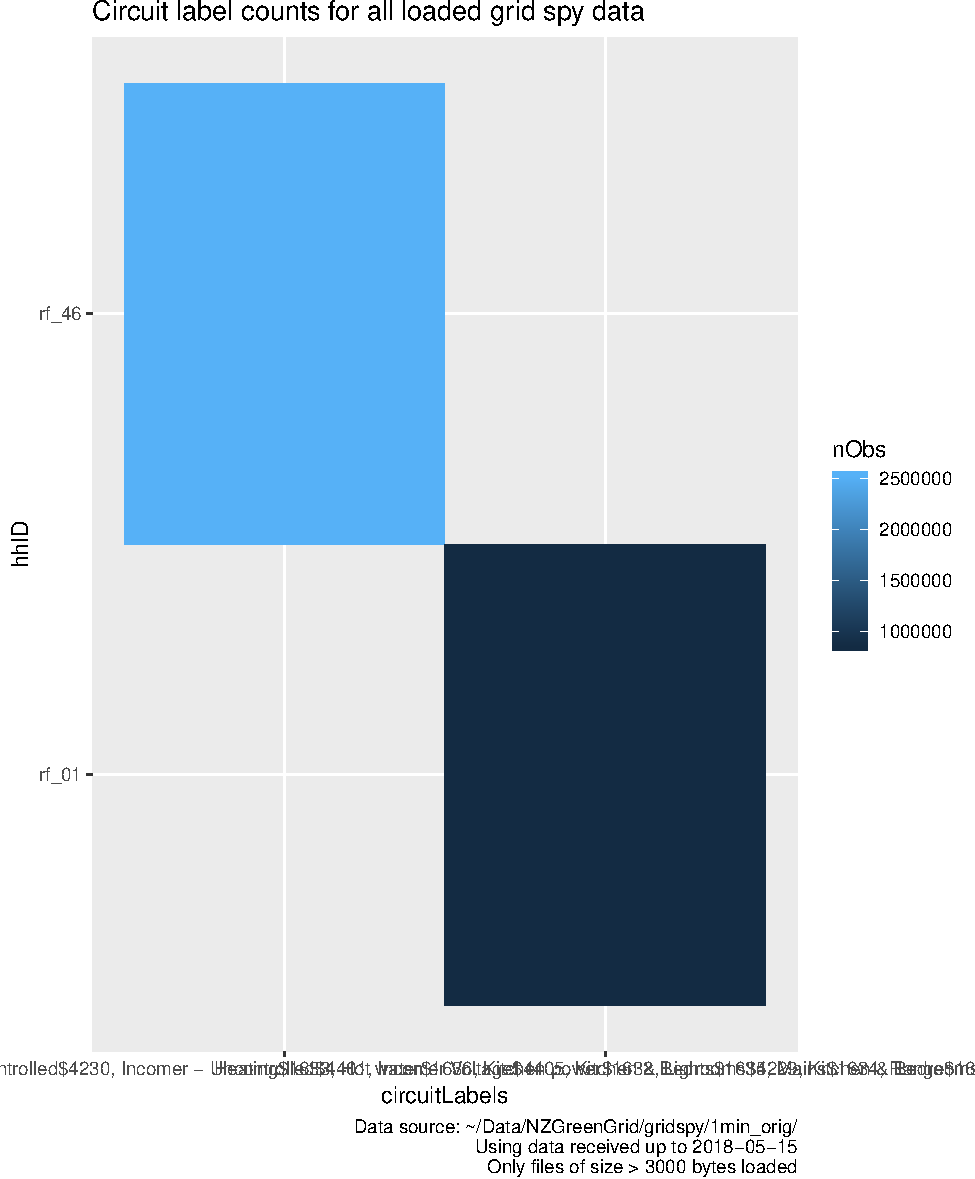
\includegraphics{processNZGGElecCons1minData_v2_files/figure-latex/plotCircuitLabelIssuesAsTile-1.pdf}

\begin{Shaded}
\begin{Highlighting}[]
\NormalTok{ggplot2}\OperatorTok{::}\KeywordTok{ggsave}\NormalTok{(}\KeywordTok{paste0}\NormalTok{(outPath, }\StringTok{"gridSpyLoadedFileCircuitLabelsPlot.png"}\NormalTok{))}
\end{Highlighting}
\end{Shaded}

\begin{verbatim}
## Saving 6.5 x 8 in image
\end{verbatim}

The following table provides more detail to aid error checking. Check
for:

\begin{itemize}
\tightlist
\item
  2+ adjacent rows which have exactly the same circuit labels but
  different hh\_ids. This implies some data from one household has been
  saved in the wrong folder;
\item
  2+ adjacent rows which have different circuit labels but identical
  hh\_ids. This could imply the same thing but is more likely to be
  errors/changes to the circuit labelling.
\end{itemize}

If the above plot and this table flag a lot of errors then some
re-naming of the circuit labels (column names) may be necessary.

\begin{Shaded}
\begin{Highlighting}[]
\NormalTok{knitr}\OperatorTok{::}\KeywordTok{kable}\NormalTok{(}\DataTypeTok{caption =} \StringTok{"Circuit labels by household with addiitonal meta-data"}\NormalTok{, t)}
\end{Highlighting}
\end{Shaded}

\begin{longtable}[]{@{}llrllllr@{}}
\caption{Circuit labels by household with addiitonal
meta-data}\tabularnewline
\toprule
circuitLabels & hhID & nFiles & minObsDate & maxObsDate & minFileDate &
maxFileDate & nObs\tabularnewline
\midrule
\endfirsthead
\toprule
circuitLabels & hhID & nFiles & minObsDate & maxObsDate & minFileDate &
maxFileDate & nObs\tabularnewline
\midrule
\endhead
Heat Pumps (2x) \& Power\$4232, Heat Pumps (2x) \& Power\$4399, Hot
Water - Controlled\$4231, Hot Water - Controlled\$4400, Incomer -
Uncontrolled\$4230, Incomer - Uncontrolled\$4401, Incomer Voltage\$4405,
Kitchen \& Bedrooms\$4229, Kitchen \& Bedrooms\$4402, Laundry \&
Bedrooms\$4228, Laundry \& Bedrooms\$4403, Lighting\$4233,
Lighting\$4404 & rf\_46 & 411 & 2015-03-26 & 2018-02-19 & 2016-06-08 &
2018-02-21 & 2529107\tabularnewline
Heating\$1633, Hot water\$1636, Kitchen power\$1632, Lights\$1635,
Mains\$1634, Range\$1637 & rf\_01 & 3 & 2014-01-05 & 2015-10-20 &
2016-09-20 & 2016-09-30 & 855836\tabularnewline
\bottomrule
\end{longtable}

Things to note:

\begin{itemize}
\tightlist
\item
  rf\_25 has an aditional unexpected ``Incomer 1 - Uncontrolled\$2757''
  circuit in some files but it's value is always NA
\end{itemize}

\subsection{Observations}\label{observations}

The following plots show the number of observations per day per
household. In theory we should not see:

\begin{itemize}
\tightlist
\item
  dates before 2014 or in to the future. These may indicate:

  \begin{itemize}
  \tightlist
  \item
    date conversion errors;
  \end{itemize}
\item
  more than 1440 observations per day. These may indicate:

  \begin{itemize}
  \tightlist
  \item
    duplicate time stamps - i.e.~they have the same time stamps but
    different power (W) values or different circuit labels;
  \item
    observations from files that are in the `wrong' rf\_XX folder and so
    are included in the `wrong' household as `duplicate' time stamps.
  \end{itemize}
\end{itemize}

If present both of the latter may have been implied by the table above
and would have evaded the de-duplication filter which simply checks each
complete row against all others within it's consolidated household
dataset (a \emph{within household absolute duplicate} check).

\begin{Shaded}
\begin{Highlighting}[]
\CommentTok{# short cut if already generated}
\CommentTok{# hhStatDT <- as.data.table(read_csv(ofile)) # parses dates}

\CommentTok{# tile plot ----}
\NormalTok{ggplot2}\OperatorTok{::}\KeywordTok{ggplot}\NormalTok{(hhStatDT, }\KeywordTok{aes}\NormalTok{( }\DataTypeTok{x =}\NormalTok{ date, }\DataTypeTok{y =}\NormalTok{ hhID, }\DataTypeTok{fill =}\NormalTok{ nObs)) }\OperatorTok{+}
\StringTok{  }\KeywordTok{geom_tile}\NormalTok{() }\OperatorTok{+}
\StringTok{  }\KeywordTok{scale_fill_gradient}\NormalTok{(}\DataTypeTok{low =} \StringTok{"red"}\NormalTok{, }\DataTypeTok{high =} \StringTok{"green"}\NormalTok{) }\OperatorTok{+}
\StringTok{  }\KeywordTok{scale_x_date}\NormalTok{(}\DataTypeTok{date_labels =} \StringTok{"%Y %b"}\NormalTok{, }\DataTypeTok{date_breaks =} \StringTok{"6 months"}\NormalTok{) }\OperatorTok{+}
\StringTok{  }\KeywordTok{theme}\NormalTok{(}\DataTypeTok{axis.text.x =} \KeywordTok{element_text}\NormalTok{(}\DataTypeTok{angle =} \DecValTok{90}\NormalTok{, }\DataTypeTok{vjust =} \FloatTok{0.5}\NormalTok{, }\DataTypeTok{hjust =} \FloatTok{0.5}\NormalTok{)) }\OperatorTok{+}\StringTok{ }
\StringTok{  }\KeywordTok{labs}\NormalTok{(}\DataTypeTok{title =} \StringTok{"N observations per household per day for all loaded grid spy data"}\NormalTok{,}
       \DataTypeTok{caption =} \KeywordTok{paste0}\NormalTok{(myCaption,}
                        \StringTok{"}\CharTok{\textbackslash{}n}\StringTok{Only files of size > "}\NormalTok{, dataThreshold, }\StringTok{" bytes loaded"}\NormalTok{)}
       
\NormalTok{  )}
\end{Highlighting}
\end{Shaded}

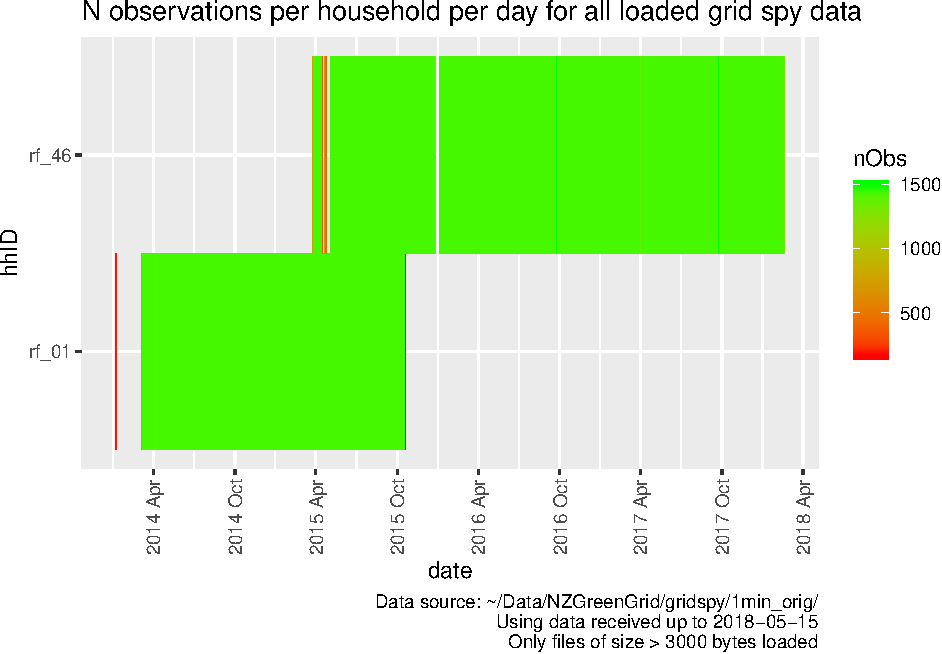
\includegraphics{processNZGGElecCons1minData_v2_files/figure-latex/loadedFilesObsPlots-1.pdf}

\begin{Shaded}
\begin{Highlighting}[]
\NormalTok{ggplot2}\OperatorTok{::}\KeywordTok{ggsave}\NormalTok{(}\KeywordTok{paste0}\NormalTok{(outPath, }\StringTok{"gridSpyLoadedFileNobsTilePlot.png"}\NormalTok{))}
\end{Highlighting}
\end{Shaded}

\begin{verbatim}
## Saving 6.5 x 4.5 in image
\end{verbatim}

\begin{Shaded}
\begin{Highlighting}[]
\CommentTok{# point plot ----}
\NormalTok{ggplot2}\OperatorTok{::}\KeywordTok{ggplot}\NormalTok{(hhStatDT, }\KeywordTok{aes}\NormalTok{( }\DataTypeTok{x =}\NormalTok{ date, }\DataTypeTok{y =}\NormalTok{ nObs, }\DataTypeTok{colour =}\NormalTok{ hhID)) }\OperatorTok{+}
\StringTok{  }\KeywordTok{geom_point}\NormalTok{() }\OperatorTok{+}
\StringTok{  }\KeywordTok{scale_x_date}\NormalTok{(}\DataTypeTok{date_labels =} \StringTok{"%Y %b"}\NormalTok{, }\DataTypeTok{date_breaks =} \StringTok{"6 months"}\NormalTok{) }\OperatorTok{+}
\StringTok{  }\KeywordTok{theme}\NormalTok{(}\DataTypeTok{axis.text.x =} \KeywordTok{element_text}\NormalTok{(}\DataTypeTok{angle =} \DecValTok{90}\NormalTok{, }\DataTypeTok{vjust =} \FloatTok{0.5}\NormalTok{, }\DataTypeTok{hjust =} \FloatTok{0.5}\NormalTok{)) }\OperatorTok{+}\StringTok{ }
\StringTok{  }\KeywordTok{labs}\NormalTok{(}\DataTypeTok{title =} \StringTok{"N observations per household per day for all loaded grid spy data"}\NormalTok{,}
       \DataTypeTok{caption =} \KeywordTok{paste0}\NormalTok{(myCaption,}
                        \StringTok{"}\CharTok{\textbackslash{}n}\StringTok{Only files of size > "}\NormalTok{, dataThreshold, }\StringTok{" bytes loaded"}\NormalTok{)}
       
\NormalTok{  )}
\end{Highlighting}
\end{Shaded}

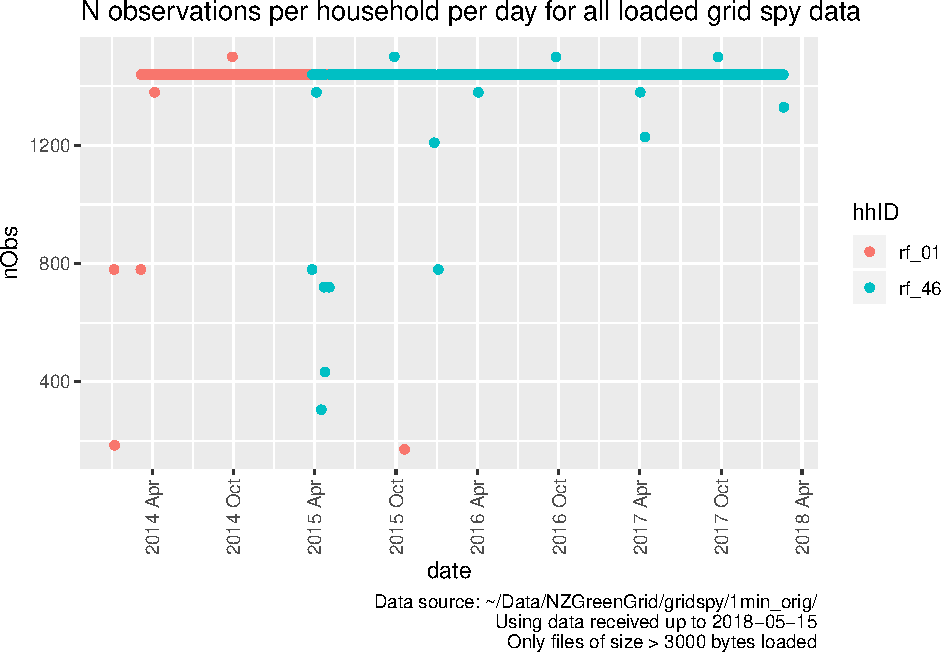
\includegraphics{processNZGGElecCons1minData_v2_files/figure-latex/loadedFilesObsPlots-2.pdf}

\begin{Shaded}
\begin{Highlighting}[]
\NormalTok{ggplot2}\OperatorTok{::}\KeywordTok{ggsave}\NormalTok{(}\KeywordTok{paste0}\NormalTok{(outPath, }\StringTok{"gridSpyLoadedFileNobsPointPlot.png"}\NormalTok{))}
\end{Highlighting}
\end{Shaded}

\begin{verbatim}
## Saving 6.5 x 4.5 in image
\end{verbatim}

The following table shows the min/max observations per day and min/max
dates for each household. As above, we should not see:

\begin{itemize}
\tightlist
\item
  dates before 2014 or in to the future (indicates date conversion
  errors)
\item
  more than 1440 observations per day (indicates potentially duplicate
  observations)
\item
  non-integer counts of circuits as it suggests some column errors
\end{itemize}

We should also not see NA in any row (indicates date conversion errors).

If we do see any of these then we still have data cleaning work to do!

\begin{Shaded}
\begin{Highlighting}[]
\CommentTok{# Stats table (so we can pick out the dateTime errors)}
\NormalTok{t <-}\StringTok{ }\NormalTok{hhStatDT[, .(}\DataTypeTok{minObs =} \KeywordTok{min}\NormalTok{(nObs),}
             \DataTypeTok{maxObs =} \KeywordTok{max}\NormalTok{(nObs), }\CommentTok{# should not be more than 1440, if so suggests duplicates}
             \DataTypeTok{meanNDataColumns =}\KeywordTok{mean}\NormalTok{(nDataColumns), }\CommentTok{#i.e. n circuits}
             \DataTypeTok{minDate =} \KeywordTok{min}\NormalTok{(date),}
             \DataTypeTok{maxDate =} \KeywordTok{max}\NormalTok{(date)),}
\NormalTok{         keyby =}\StringTok{ }\NormalTok{.(hhID)]}

\NormalTok{knitr}\OperatorTok{::}\KeywordTok{kable}\NormalTok{(}\DataTypeTok{caption =} \StringTok{"Summary observation stats by hhID"}\NormalTok{, t)}
\end{Highlighting}
\end{Shaded}

\begin{longtable}[]{@{}lrrrll@{}}
\caption{Summary observation stats by hhID}\tabularnewline
\toprule
hhID & minObs & maxObs & meanNDataColumns & minDate &
maxDate\tabularnewline
\midrule
\endfirsthead
\toprule
hhID & minObs & maxObs & meanNDataColumns & minDate &
maxDate\tabularnewline
\midrule
\endhead
rf\_01 & 171 & 1500 & 6 & 2014-01-05 & 2015-10-20\tabularnewline
rf\_46 & 305 & 1500 & 13 & 2015-03-26 & 2018-02-19\tabularnewline
\bottomrule
\end{longtable}

Finally we show the total number of households which we think are still
sending data.

\begin{Shaded}
\begin{Highlighting}[]
\NormalTok{plotDT <-}\StringTok{ }\NormalTok{hhStatDT[, .(}\DataTypeTok{nHH =} \KeywordTok{uniqueN}\NormalTok{(hhID)), keyby =}\StringTok{ }\NormalTok{.(date)]}

\CommentTok{# point plot ----}
\NormalTok{ggplot2}\OperatorTok{::}\KeywordTok{ggplot}\NormalTok{(plotDT, }\KeywordTok{aes}\NormalTok{( }\DataTypeTok{x =}\NormalTok{ date, }\DataTypeTok{y =}\NormalTok{ nHH)) }\OperatorTok{+}
\StringTok{  }\KeywordTok{geom_point}\NormalTok{() }\OperatorTok{+}
\StringTok{  }\KeywordTok{scale_x_date}\NormalTok{(}\DataTypeTok{date_labels =} \StringTok{"%Y %b"}\NormalTok{, }\DataTypeTok{date_breaks =} \StringTok{"6 months"}\NormalTok{) }\OperatorTok{+}
\StringTok{  }\KeywordTok{theme}\NormalTok{(}\DataTypeTok{axis.text.x =} \KeywordTok{element_text}\NormalTok{(}\DataTypeTok{angle =} \DecValTok{90}\NormalTok{, }\DataTypeTok{vjust =} \FloatTok{0.5}\NormalTok{, }\DataTypeTok{hjust =} \FloatTok{0.5}\NormalTok{)) }\OperatorTok{+}\StringTok{ }
\StringTok{  }\KeywordTok{labs}\NormalTok{(}\DataTypeTok{title =} \StringTok{"N live households per day for all loaded grid spy data"}\NormalTok{,}
       \DataTypeTok{caption =} \KeywordTok{paste0}\NormalTok{(myCaption,}
                        \StringTok{"}\CharTok{\textbackslash{}n}\StringTok{Only files of size > "}\NormalTok{, dataThreshold, }\StringTok{" bytes loaded"}\NormalTok{)}
       
\NormalTok{  )}
\end{Highlighting}
\end{Shaded}

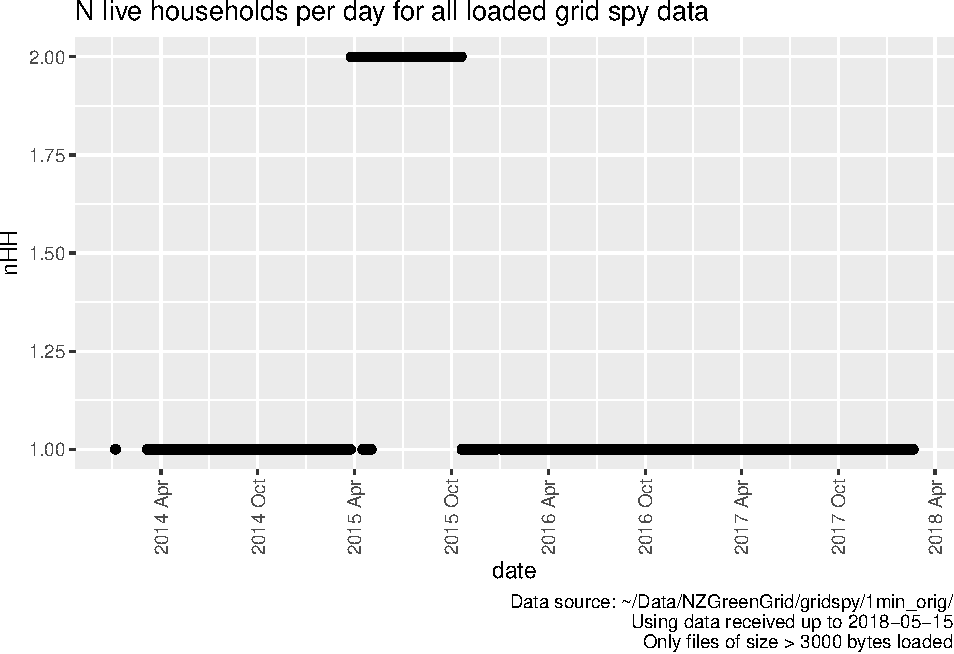
\includegraphics{processNZGGElecCons1minData_v2_files/figure-latex/liveDataHouseholds-1.pdf}

\begin{Shaded}
\begin{Highlighting}[]
\NormalTok{ggplot2}\OperatorTok{::}\KeywordTok{ggsave}\NormalTok{(}\KeywordTok{paste0}\NormalTok{(outPath, }\StringTok{"gridSpyLiveHouseholdsToDate.png"}\NormalTok{))}
\end{Highlighting}
\end{Shaded}

\begin{verbatim}
## Saving 6.5 x 4.5 in image
\end{verbatim}

\section{Runtime}\label{runtime}

\begin{Shaded}
\begin{Highlighting}[]
\NormalTok{t <-}\StringTok{ }\KeywordTok{proc.time}\NormalTok{() }\OperatorTok{-}\StringTok{ }\NormalTok{startTime}

\NormalTok{elapsed <-}\StringTok{ }\NormalTok{t[[}\DecValTok{3}\NormalTok{]]}
\end{Highlighting}
\end{Shaded}

Analysis completed in 356.022 seconds ( 5.93 minutes) using
\href{https://cran.r-project.org/package=knitr}{knitr} in
\href{http://www.rstudio.com}{RStudio} with R version 3.4.4 (2018-03-15)
running on x86\_64-apple-darwin15.6.0.

\section{R environment}\label{r-environment}

R packages used:

\begin{itemize}
\tightlist
\item
  base R - for the basics (R Core Team 2016)
\item
  data.table - for fast (big) data handling (Dowle et al. 2015)
\item
  lubridate - date manipulation (Grolemund and Wickham 2011)
\item
  ggplot2 - for slick graphics (Wickham 2009)
\item
  readr - for csv reading/writing (Wickham, Hester, and Francois 2016)
\item
  dplyr - for select and contains (Wickham and Francois 2016)
\item
  progress - for progress bars (Csárdi and FitzJohn 2016)
\item
  knitr - to create this document \& neat tables (Xie 2016)
\item
  kableExtra - for extra neat tables (Zhu 2018)
\item
  nzGREENGrid - for local NZ GREEN Grid project utilities
\end{itemize}

\begin{Shaded}
\begin{Highlighting}[]
\KeywordTok{sessionInfo}\NormalTok{()}
\end{Highlighting}
\end{Shaded}

\begin{verbatim}
## R version 3.4.4 (2018-03-15)
## Platform: x86_64-apple-darwin15.6.0 (64-bit)
## Running under: macOS High Sierra 10.13.4
## 
## Matrix products: default
## BLAS: /Library/Frameworks/R.framework/Versions/3.4/Resources/lib/libRblas.0.dylib
## LAPACK: /Library/Frameworks/R.framework/Versions/3.4/Resources/lib/libRlapack.dylib
## 
## locale:
## [1] en_GB.UTF-8/en_GB.UTF-8/en_GB.UTF-8/C/en_GB.UTF-8/en_GB.UTF-8
## 
## attached base packages:
## [1] stats     graphics  grDevices utils     datasets  methods   base     
## 
## other attached packages:
## [1] progress_1.1.2      dplyr_0.7.4         readr_1.1.1        
## [4] lubridate_1.7.4     data.table_1.10.4-3 kableExtra_0.8.0   
## [7] knitr_1.20          ggplot2_2.2.1.9000  nzGREENGrid_0.1.0  
## 
## loaded via a namespace (and not attached):
##  [1] Rcpp_0.12.16      highr_0.6         bindr_0.1.1      
##  [4] pillar_1.2.2      compiler_3.4.4    plyr_1.8.4       
##  [7] prettyunits_1.0.2 tools_3.4.4       digest_0.6.15    
## [10] evaluate_0.10.1   tibble_1.4.2      gtable_0.2.0     
## [13] viridisLite_0.3.0 pkgconfig_2.0.1   rlang_0.2.0.9001 
## [16] rstudioapi_0.7    yaml_2.1.18       bindrcpp_0.2.2   
## [19] withr_2.1.2       stringr_1.3.0     httr_1.3.1       
## [22] xml2_1.2.0        hms_0.4.2         rprojroot_1.3-2  
## [25] grid_3.4.4        glue_1.2.0        R6_2.2.2         
## [28] rmarkdown_1.9     magrittr_1.5      backports_1.1.2  
## [31] scales_0.5.0.9000 htmltools_0.3.6   assertthat_0.2.0 
## [34] rvest_0.3.2       colorspace_1.3-2  labeling_0.3     
## [37] stringi_1.1.7     lazyeval_0.2.1    munsell_0.4.3
\end{verbatim}

\section*{References}\label{references}
\addcontentsline{toc}{section}{References}

\hypertarget{refs}{}
\hypertarget{ref-progress}{}
Csárdi, Gábor, and Rich FitzJohn. 2016. \emph{Progress: Terminal
Progress Bars}. \url{https://CRAN.R-project.org/package=progress}.

\hypertarget{ref-data.table}{}
Dowle, M, A Srinivasan, T Short, S Lianoglou with contributions from R
Saporta, and E Antonyan. 2015. \emph{Data.table: Extension of
Data.frame}. \url{https://CRAN.R-project.org/package=data.table}.

\hypertarget{ref-lubridate}{}
Grolemund, Garrett, and Hadley Wickham. 2011. ``Dates and Times Made
Easy with lubridate.'' \emph{Journal of Statistical Software} 40 (3):
1--25. \url{http://www.jstatsoft.org/v40/i03/}.

\hypertarget{ref-baseR}{}
R Core Team. 2016. \emph{R: A Language and Environment for Statistical
Computing}. Vienna, Austria: R Foundation for Statistical Computing.
\url{https://www.R-project.org/}.

\hypertarget{ref-ggplot2}{}
Wickham, Hadley. 2009. \emph{Ggplot2: Elegant Graphics for Data
Analysis}. Springer-Verlag New York. \url{http://ggplot2.org}.

\hypertarget{ref-dplyr}{}
Wickham, Hadley, and Romain Francois. 2016. \emph{Dplyr: A Grammar of
Data Manipulation}. \url{https://CRAN.R-project.org/package=dplyr}.

\hypertarget{ref-readr}{}
Wickham, Hadley, Jim Hester, and Romain Francois. 2016. \emph{Readr:
Read Tabular Data}. \url{https://CRAN.R-project.org/package=readr}.

\hypertarget{ref-knitr}{}
Xie, Yihui. 2016. \emph{Knitr: A General-Purpose Package for Dynamic
Report Generation in R}. \url{https://CRAN.R-project.org/package=knitr}.

\hypertarget{ref-kableExtra}{}
Zhu, Hao. 2018. \emph{KableExtra: Construct Complex Table with 'Kable'
and Pipe Syntax}. \url{https://CRAN.R-project.org/package=kableExtra}.


\end{document}
